% One-site TDVP, the forward half of a step: the effective Hamiltonian of the
% site the centre is on, applied to the centre.
%
% The state is in mixed canonical form with its centre AC on this site, so
% everything to the left of it contracts into L and everything to the right
% into R, and the tensor-network part of the Schroedinger equation is local:
% i dAC/dt is this picture. The integrator exponentiates it, AC moves one
% step, and the sweep goes on.
%
% The bra layer is empty, and its three indices are the free ones -- the
% result is a tensor shaped like AC, which is what an equation for AC needs.
% Each ends at the border the tensor in that slot would have.
\documentclass[border=4pt]{standalone}
\usepackage{amsmath,amssymb}
\usepackage{tikz-tensors}
\begin{document}
\begin{tikzpicture}
  \tnstack[left=$L$, right=$R$]{H}{1}{ket, op, bra}
  \tnlayer{H}{ket}{centre/$A_C$}
  \tnlayer{H}{op}{mpo/$W$}
  \tnconnect{H}
  \tnopen{down}{H-op-1}
  \tnput[below]{H-left-bra}{$a$}
  \tnput[below]{H-op-1-down}{$\sigma$}
  \tnput[below]{H-right-bra}{$b$}
\end{tikzpicture}
\end{document}
